
\begin{frame}{Tarides}

    \begin{itemize}[label=$-$]
        \item on fait des logiciels et du service en OCaml
        \item 70 employés (France, UK, USA, Inde etc..)
        \item tout en open source !  
    \end{itemize}
    
\begin{columns} 
    \column{0.3\linewidth} 
    \centering
    
\includegraphics[width=\textwidth]{slides/images/logo-TARIDES.png}

    \column{0.5\linewidth}
    \centering
    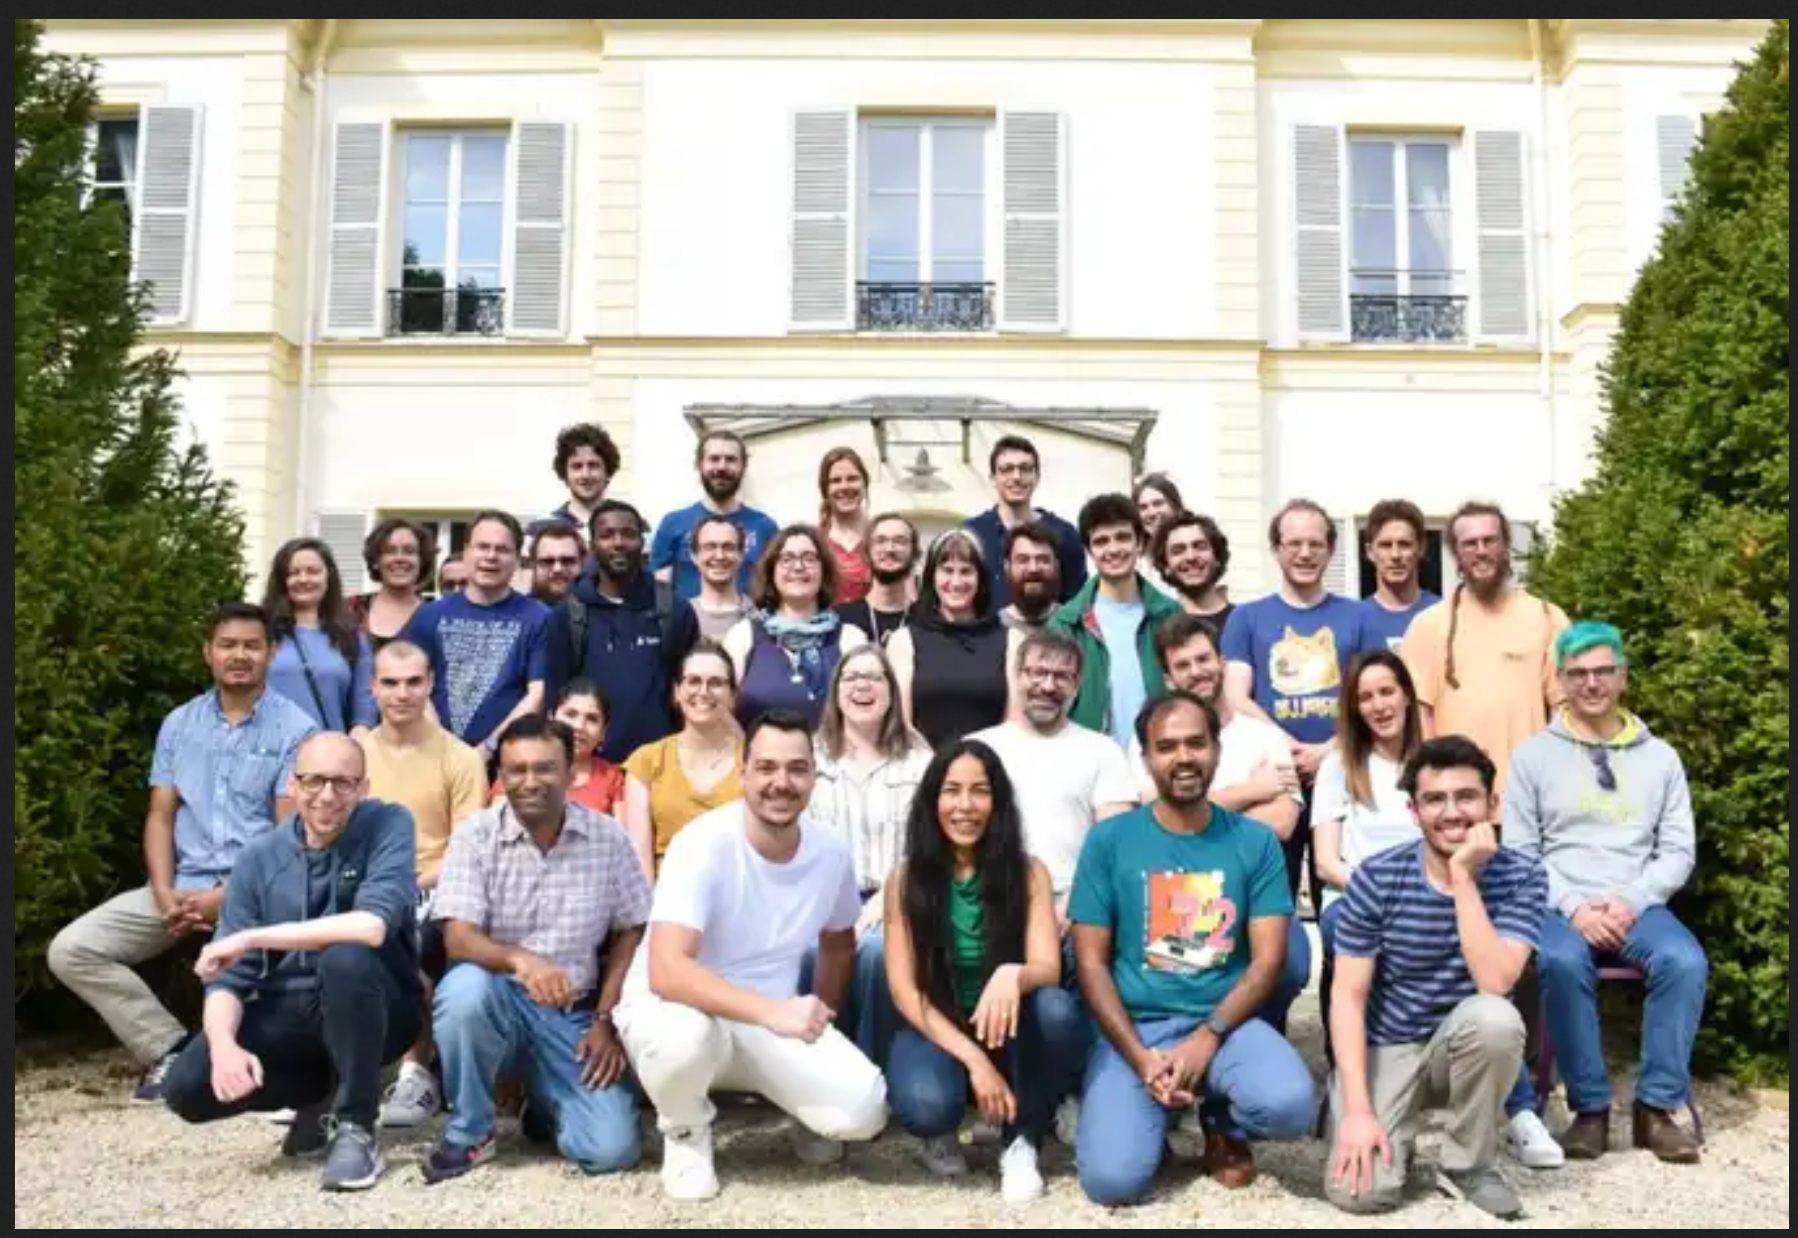
\includegraphics[width=\textwidth]{slides/images/tarides_team.png}
\end{columns}

\end{frame}

\begin{frame}{Plan}
   \subtt{Programmation système en OCaml} 
   
   \ding{217} autour de l'écriture d'un "mini" shell :
    \begin{itemize}[label=\ding{114}]
        \item le module Unix
        \item les processus Unix  
        \item et plus
    \end{itemize}   
    
    \ding{217} les algos d'exclusion mutuelle en OCaml

    \subtt{OCaml dans la vraie vie} 
     \begin{itemize}[label=$-$]
        \item Mirage : \textbf{un} système en OCaml
        \item QCheck : un vérificateur de propriétés automatiques
        \item OCaml 5.0
        \item Écosystème OCaml
    \end{itemize}   
\end{frame}